\chapter{Hardware und Software}
\renewcommand{\chaptertitle}{Hardware und Software}

\lehead[]{\sf\hspace*{-2.00cm}\textcolor{white}{\colorbox{lightblue}{\makebox[1.60cm][r]{\thechapter}}}\hspace{0.17cm}\textcolor{lightblue}{\chaptertitle}}
\rohead[]{\textcolor{lightblue}{\chaptertitle}\sf\hspace*{0.17cm}\textcolor{white}{\colorbox{lightblue}{\makebox[1.60cm][l]{\thechapter}}}\hspace{-2.00cm}}
%\chead[]{}
\rehead[]{\textcolor{lightblue}{AvHG, Inf, My}}
\lohead[]{\textcolor{lightblue}{AvHG, Inf, My}}


\section{Hardware}

\subsection{Grundstruktur eines Computers}

Um von den elektrischen Vorgängen in einem Rechner abstrahieren zu können, ist
es zweckmäßig, den Rechner als Datenverarbeiter anzusehen. Die Verarbeitung von
Daten funktioniert nach dem sogenannten EVA-Prinzip:

\begin{figure}[h]
  \centering
   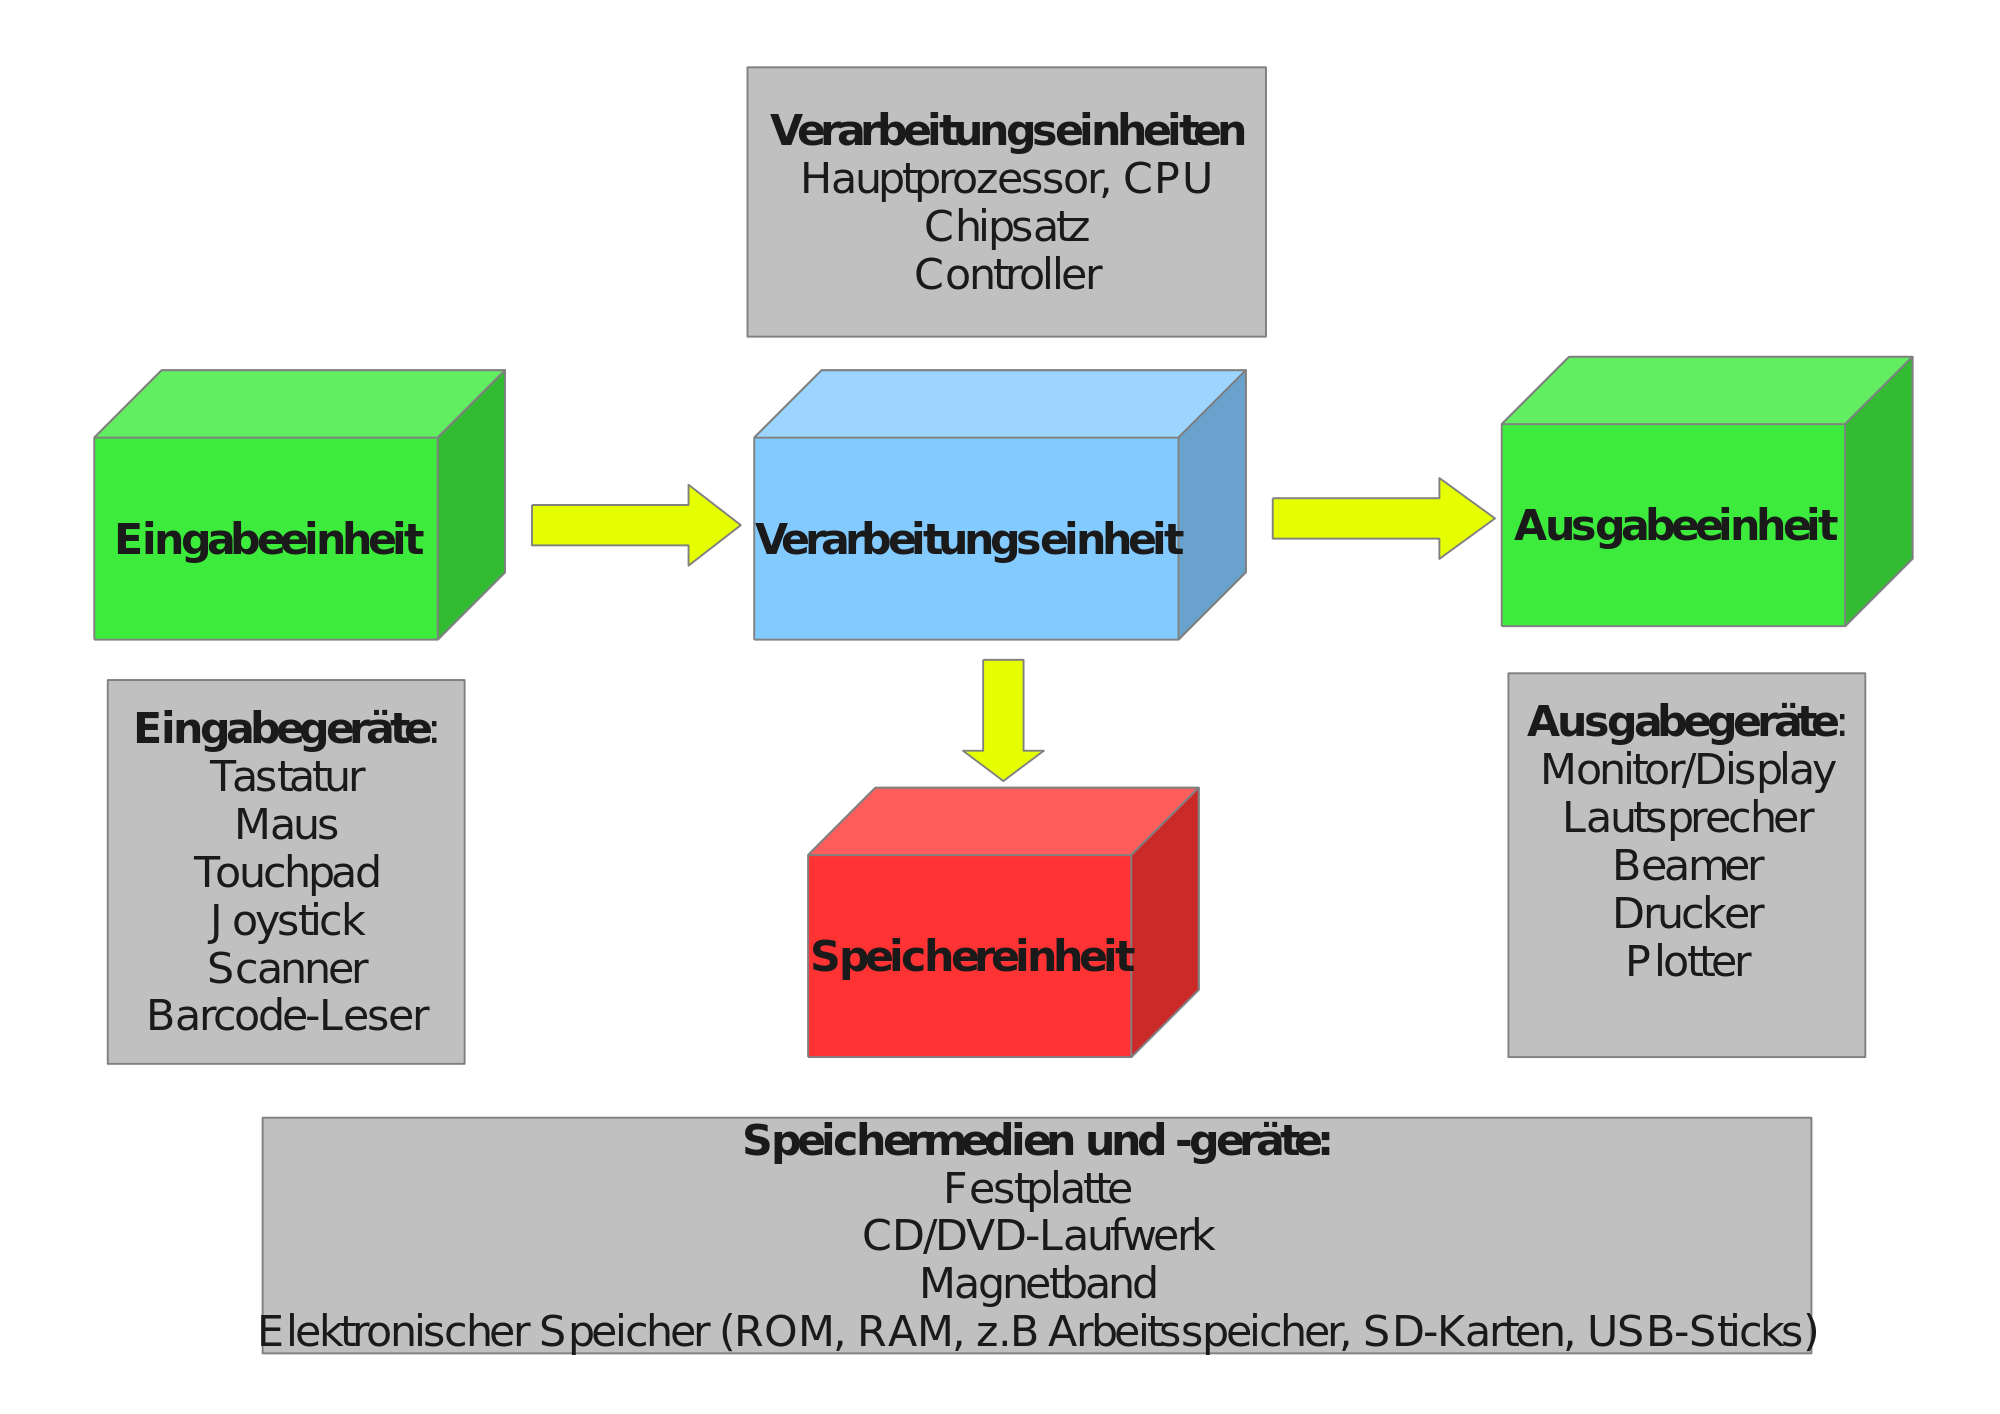
\includegraphics[width=1.0\textwidth]{./inf/SEKII/02_Hardware_und_Software/EVA.png}
\end{figure}
% http://commons.wikimedia.org/wiki/File:EVA-Prinzip.svg

Der Computer besteht vereinfacht aus drei Einheiten:

\begin{compactitem}
\item Ein-/Ausgabegeräte
\item Hauptspeicher (engl. RAM = Random Access Memory)
\item Prozessor (engl. CPU = Central Processing Unit)
\end{compactitem}

Die Einheiten werden durch Datenleitungen miteinander verbunden, die man als Bus bezeichnet.

\begin{figure}[h]
  \centering
   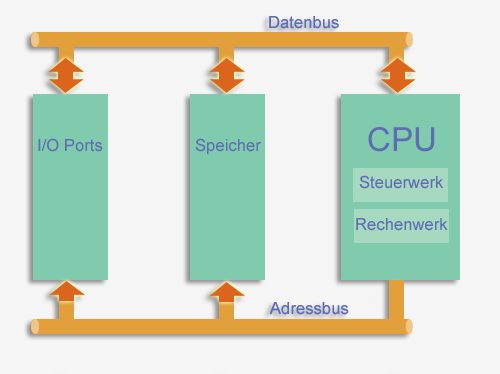
\includegraphics[width=0.5\textwidth]{./inf/SEKII/02_Hardware_und_Software/Bus.png}
\end{figure}
% http://www.neogrid.de/was-ist/CPU
% http://www.neogrid.de/nutzungsbedingungen.php

\subsubsection{Eingabe und Ausgabegeräte}

Die Eingabe- und Ausgabegeräte haben die Aufgabe, die zu verarbeitenden Daten
von der Außenwelt in den Hauptspeicher zu übertragen, bzw. die Ergebnisse der
Verarbeitung wieder in die Außenwelt zu bringen. Solche Geräte werden auch
Peripheriegeräte genannt. (Peripherie = Umgebung; Rand)

\subsubsection{Hauptspeicher (RAM)}

Die Aufgabe des Hauptspeichers ist es, alle aktuell benötigten
Daten zu speichern. Dazu gehört auch der Programmcode der
momentan laufenden Programme.

Um Daten in den Hauptspeicher zu schreiben bzw. von dort zu
lesen, sind die Speicherzellen des Hauptspeichers
durchnummeriert. Jede Speicherzelle hat eine eindeutige
Nummer, die sogenannte Adresse, mit der man sie ansprechen
kann. Bei einem Zugriff auf den Hauptspeicher transportiert der
Adressbus die gewünschte Adresse und der Datenbus die Daten.

\subsubsection{Prozessor (CPU)}

Die CPU ist das \glqq Gehirn\grqq\ des Rechners. Sie hat die Aufgabe, die Daten,
die im Hauptspeicher liegen, zu verarbeiten, d.h.\ sie zu lesen, mit ihrer Hilfe
Berechnungen durchzuführen und die Berechnungsergebnisse in den Hauptspeicher
zu schreiben.

Die CPU lädt die Kommandos eines Programms Schritt für Schritt aus dem
Hauptspeicher und führt sie nacheinander aus. Der Hauptspeicher unterscheidet
nicht zwischen Daten und Programmen. Erst durch die CPU wird eine Datenfolge im
Hauptspeicher zu einem Programm.

Die Leistungsfähigkeit eines Computers ist unter anderem davon abhängig, wie
schnell die Befehle vom Prozessor abgearbeitet werden. Der Prozessor ist mit
einer Uhr verbunden, die ihn in gewissen Zeitabständen anweist, den nächsten
Befehl aus dem Hauptspeicher zu holen und auszuführen. Je schneller dieser
Uhrtakt schlägt, desto schneller wird auch der Computer arbeiten. Ein Gigahertz
entspricht 1.000.000.000 Stromimpulsen pro Sekunde.

\subsubsection{Adress- und Datenbus}

Der Datenbus überträgt die eigentlichen Daten zwischen den Geräten, wie z.B.\
Bilder, Texte, Programmcode usw. Über den Adressbus übermittelt die CPU die
Speicheradressen, an denen sich die zu transportierenden Daten befinden. Auf
diese Weise steuert die CPU, welche Daten übertragen werden sollen.

\subsection{Speicherarten}

Aufwändige Aufgaben, wie z.B. die Wettervorhersage, beruhen auf der
Verarbeitung von Millionen von Messdaten. Durch die immens gesteigerte
Verarbeitungsgeschwindigkeit der Computer während der letzten Jahre, können
immer komplexere Probleme durch Computer berechnet werden. Die ersten Rechner
benötigten einige Sekunden, um eine Addition von zwei ganzen Zahlen
durchzuführen, heutige CPUs führen einige hundert Millionen Rechenoperationen
pro Sekunde durch.

Der Speicher im Computer muss in der Lage sein, die CPU mit der entsprechenden
Geschwindigkeit mit Daten zu versorgen und er muss möglichst viele Daten
speichern können. Die Speicherbausteine, die mit der Geschwindigkeit der CPU
mithalten können, haben allerdings zwei Nachteile: Sie sind teuer und sie sind
flüchtig, d.h.\ sie können die Daten nur speichern, solange sie mit Strom
versorgt werden.

\begin{minipage}{1.0\textwidth}
Deshalb gibt es in einem Computer verschiedene Arten von Speichern:

\begin{compactitem}
\item In der CPU gibt es spezielle Speicherzellen, sogenannte \emph{Register},
die dazu dienen, die Operanden der gerade ausgeführten Anweisung zu halten. Die
Register sind Teil des CPU-Kernes, d.h.\ ebenso schnell wie die CPU, und ändern
ihren Inhalt teilweise nach jeder Anweisung. Ein Register speichert ein
Computer-„Wort“ (heutzutage je nach CPU 32 bis 128 Bit).

\item Der schnelle \emph{Hauptspeicher} (englisch \emph{RAM} = \emph{Random
Access Memory}) speichert die Daten, die für die laufenden Programme benötigt
werden. Der Hauptspeicher ist über den Adress- und Datenbus direkt mit der CPU
verbunden. Da Hauptspeicher teuer ist, kann dieser Speicher nicht beliebig groß
sein.

\item Alle anderen Daten (und Programme) werden in sogenannten
\emph{Hintergrundspeichern} gehalten (Festplatte, CD-ROM-Laufwerk, USB-Stick,
usw.). Hintergrundspeicher sind langsamer als Hauptspeicher, billiger, meist
deutlich größer und nicht flüchtig.

\item Moderne CPUs sind vom Hauptspeicher durch sogenannte \emph{Caches}
entkoppelt. Caches sind schneller (und teurer) als Hauptspeicher und haben die
Aufgabe häufig benötigte Bereiche des Hauptspeichers zwischen zu lagern, um so
die CPU möglichst unabhängig von der Geschwindigkeit des Hauptspeichers zu
machen.
\end{compactitem}
\end{minipage}